\subsubsection{}
The heuristic used for the Minimax player is
%based on the \lstinline!State.evaluation()! method shown in Lst. \ref{lst:evaluation}.
%
%\begin{lstlisting}[language=Python, label={lst:evaluation}, caption={Evaluation function for the heuristic of the Minimax player.}]
%    def evaluation(self, turn: int):
%    coefficient_array = np.full(8, 0)
%        if turn < 18:
%        coefficient_array = np.array([18, 26, 1, 9, 10, 7, 0, 0])
%        elif turn >= 18:
%        coefficient_array = np.array([30, 31, 10, 11, 5, 0.5, 8, 1086])
%        # if turn >= 25:
%        #     coefficient_array = np.array([25, 35, 7, 11, 5, 0.5, 8, 1150])
%        # compute the values of the various heuristics
%        r1 = self.r1()
%        r2, r5, r6, r7 = self.r2r5r6r7()
%        r3, r8 = self.r3r8()
%        r4 = self.r4()
%        # r8 = self.r8()
%        r_array = np.array([r1, r2, r3, r4, r5, r6, r7, r8])
%        return (np.multiply(coefficient_array, r_array)).sum()
%
%    def r1(self):
%        """
%        Returns:
%        1 if the player closed a mill in the last move;
%        -1 if the rival closed a mill in the last move;
%        0 otherwise.
%        :return: int, values are (1, 0, -1)
%        """
%        return self.is_mill_closed
%
%    def r2r5r6r7(self):
%        """
%        Computes evaluation functions R2, R6, R7.
%        R2 counts the number of closed mills.
%        R5 counts the number of 2-piece configurations (a piece can be added in a cell to close a mill).
%        R6 counts the number of 3-piece configurations (a piece can be added in two different positions to close a morris).
%        R7 counts the number of double mills.
%        :return: r2, r6, r7 (tuple of three int items)
%        """
%        mill_combinations = [[0, 1, 2], [0, 3, 5], [2, 4, 7], [5, 6, 7], [1, 9, 17], [8, 9, 10], [10, 12, 15],
%        [13, 14, 15], [8, 11, 13], [16, 17, 18], [18, 20, 23], [16, 19, 21], [21, 22, 23],
%        [3, 11, 19], [20, 12, 4], [6, 14, 22]]
%        mine_mill = list()
%        rival_mill = list()
%        mine_tris = list()
%        rival_tris = list()
%        r2 = 0
%        r5 = 0
%        r6 = 0
%        r7 = 0
%
%        # R2, R6
%        for mill in mill_combinations:
%        # R2
%        if self.board[mill[0]] == self.board[mill[1]] == self.board[mill[2]]:
%        if self.board[mill[0]] == 1:
%        r2 += 1
%        mine_mill = mine_mill + mill
%        else:
%        r2 -= 1
%        rival_mill = rival_mill + mill
%        # R6 first part
%        # tris is a 2-piece configuration, i.e. when you have two soldiers and a void cell in a row.
%        # We collect them in two lists the same way we do with mills.
%        else:
%        # tris contains the values of three cells in a row.
%        # mine_tris and rival_tris contain a list of cells where soldiers of player or rival are and are
%        # candidate tris for the 3-piece configurations
%        tris = self.board[mill].tolist()
%        # if it is a candidate for the player
%        if tris.count(1) == 2 and tris.count(0) == 1:
%        index_0 = tris.index(0)
%        mill.pop(index_0)
%        mine_tris = mine_tris + mill
%        # if it is a candidate for the rival
%        elif tris.count(2) == 2 and tris.count(0) == 1:
%        index_0 = tris.index(0)
%        mill.pop(index_0)
%        rival_tris = rival_tris + mill
%        # R5 first part
%        # mine_tris is a list containing all the cells included in 2-piece configurations: to each configuration,
%        # 2 items correspond. To compute a preliminary value of 2-piece configurations we will divide the length of the
%        # lists by 2. Later in the method, we will subtract twice the number of 3-piece configurations to the number of
%        # 2-piece configurations computed as preliminary value.
%        r5 = len(mine_tris) / 2 - len(rival_tris) / 2
%
%        # R7
%        # mine_mill and rival_mill are two lists, each one long n*3 items, where n is the number of mills present. If
%        # an element belongs to two mills, it should appear twice in the list.
%        for cell in range(24):
%        if mine_mill.count(cell) > 1:
%        r7 += 1
%        elif rival_mill.count(cell) > 1:
%        r7 -= 1
%
%        # R6 second part
%        for cell in range(24):
%        if mine_tris.count(cell) == 2:
%        r6 += 1
%        elif rival_tris.count(cell) == 2:
%        r6 -= 1
%        elif mine_tris.count(cell) > 2 or rival_tris.count(cell) > 2:
%        raise ValueError
%
%        # R5 second part
%        r5 = r5 - 2 * r6
%
%        return r2, r5, r6, r7
%
%    def r3r8(self):
%        """
%        Computes R3 and R8 evaluation functions.
%        R3: number of blocked soldiers of the rival minus number of blocked soldiers of my player.
%        R8: returns an int depending on the state: if the state is winning for my player (1), or for rival (-1),
%        or otherwise (0).
%        :return: R3, R8
%        """
%        # initialize variables for the enumeration
%        r3 = 0
%        r8 = 0
%        my_n_blocked_soldiers = 0
%        my_n_non_placed_soldiers = 0
%        rival_n_blocked_soldiers = 0
%        rival_n_non_placed_soldiers = 0
%
%        # R3
%        # Computation for player -------------
%        # check for each soldier in the game if it can move
%        for soldier in self.my_pos:
%        # if soldier is sill to be placed
%        if soldier == 0:
%        my_n_non_placed_soldiers += 1
%        # if soldier is on board and is blocked
%        elif soldier > 0 and not self.check_non_blocked_soldier(soldier):
%        my_n_blocked_soldiers += 1
%        # Computation for rival --------------
%        # check for each soldier in the game if it can move
%        for soldier in self.rival_pos:
%        # if soldier is still to be placed
%        if soldier == 0:
%        rival_n_non_placed_soldiers += 1
%        # if soldier is on board and is blocked
%        elif soldier > 0 and not self.check_non_blocked_soldier(soldier):
%        rival_n_blocked_soldiers += 1
%        # compute R3 value
%        r3 = rival_n_blocked_soldiers - my_n_blocked_soldiers
%
%        # R8
%        # collects np.arrays of bool: True if the soldier is alive, False if it is dead.
%        # Then it counts how many non_zero elements (non-False, i.e. alive soldiers) there are.
%        my_soldiers_alive = np.count_nonzero(self.my_pos != -2)
%        rival_soldiers_alive = np.count_nonzero(self.rival_pos != -2)
%
%        if my_soldiers_alive < 3:
%        if my_soldiers_alive != 2:
%        raise ValueError
%        # print("ValueError at R8")
%        r8 = -1
%        elif rival_soldiers_alive < 3:
%        if rival_soldiers_alive != 2:
%        # raise ValueError
%        print("ValueError at R8")
%        r8 = 1
%        # TODO: check again these following conditions
%        # if my player have 3 or more soldiers on the field or to be placed but they are blocked
%        elif my_soldiers_alive - my_n_blocked_soldiers - my_n_non_placed_soldiers <= 0:
%        r8 = -1
%        elif rival_soldiers_alive - my_n_blocked_soldiers - my_n_non_placed_soldiers <= 0:
%        r8 = 1
%
%        return r3, r8
%
%    def r4(self):
%    """
%        Compute material difference
%        :return: n. of our soldiers alive - n. of rival's soldiers alive
%        """
%        return len(np.where(self.my_pos != -2)[0]) - len(np.where(self.rival_pos != -2)[0])
%\end{lstlisting}
%
%The heuristic function is
based on 7 contributions:
\begin{itemize}
    \item R1: returns 1 if a mill was closed by our player in he last move, returns -1 if a mill was closed by the opponent n the last move, returns 0 otherwise;
    \item R2: returns the difference between the number of my player's morrises and the number of the rival's ones;
    \item R3: returns the difference between the number of my players' blocked pieces and the number of the rival's ones;
    \item R4: returns the difference between the number of my player's pieces and the number of the rival's ones;
    \item R5: returns the difference between the number of my player's 2-piece configurations and the number of the rival's ones (a 2-piece configuration is made by two soldiers and a free cell in a row), not accounting for the number of 2-piece configurations that compose the 3-piece configurations;
    \item R6: returns the difference between the number of my player's 3-piece configurations and the number of the rival's ones (a 3-piece configuration is made by two 2-piece configuration that shares a soldier);
    \item R7: returns the difference between the number of my player's double mills and the number of the rival's ones (a double mill is made by two mills that share a soldier).
\end{itemize}

In our case we set different coefficients for the two different phases of the game. For the first phase we have that the heuristic value assigned to he evaluated states is given by:
\begin{equation*}
    E(s) = 18 \times R1 + 26 \times R2 + 1 \times R3 + 9 \times R4 + 10 \times R5 + 7 \times R6 + 0 \times R7
\end{equation*}
while for the second phase of the game we have:
\begin{equation*}
    E(s) = 30 \times R1 + 31 \times R2 + 10 \times R3 + 11 \times R4 + 5 \times R5 + 0.5 \times R6 + 8 \times R7
\end{equation*}

\subsubsection{}
The Player submitted for the competition corresponds to the Alpha-beta player coded for the other exercises, with the strategy implemented for the global time management, as explained later in the section \ref{section_Ec}. No particular improvement was implemented in the heuristic, since we reckoned that the heuristic was already quite informative.

\subsubsection{}\label{section_Ec}
The runtime of the \lstinline!make_move! method was managed according to the following ideas.

\textbf{global\_time limit strategy}
We get the global time and calculation average time for single move, assuming N=35 moves:
$$
avg\_time = \frac{global\_time}{N}
$$
We want to take into account the fact that for higher turns we need less time. so we are using a turn factor function to factorize the move time.

Factor function:
\begin{itemize}
    \item We want a monotonically descending function
    \item at turn=0 we want to get $turn\_factor=1$
    \item at turn=N (the average number of moves) we want to remain with 1 second for move, i.e. $turn\_factor(N)=1/avg\_time$
    \item so we used an exponent $turn_factor(turn)=e^{-\lambda\cdot turn}$
    \item from the above conditions, easy to see that: $\lambda=-(\frac{1}{N})\ln(\frac{1}{avg\_time})$
\end{itemize}
With $move\_time$ calculated every turn we use it to set a time limit for a single turn.

\textbf{one-move\_time limit strategy}
We saw that as the turn number is higher most of the time it takes less time to perform a move. That was accounted in a Global Time strategy. In addition we saw that the difference between two adjacent  depth is around ~20. This fact is not so strange cause we know that asymptotically the time of DFS is $O(b^d)$ where
b is the branching factor and d is the depth, so asymptotically the ratio between two adjoint depth is $\sim b$ :
$$
\frac{T(depth+1)}{T(depth)}=\frac{b^{d+1}}{b}=b
$$

Fig. \ref{fig:partE_1} shows how it resulted from experiments that the time ratio of two adjacent depths is bound by 25.

Our code strategy:
\begin{itemize}
    \item Every depth we measure the time it took to perform the Minimax or Alpha-beta loop ($iter\_time$)
    \item We continue to the next depth if the $remain\_time\ >\ 40\cdot iter\_time$
    \item We took the factor of 40 (to be on the safe side)
    \item o	In addition, we took safety factors of few seconds to be sure that we have enough time to send our move to the game\_wrapper
\end{itemize}

\begin{figure}[H]
    \centering
    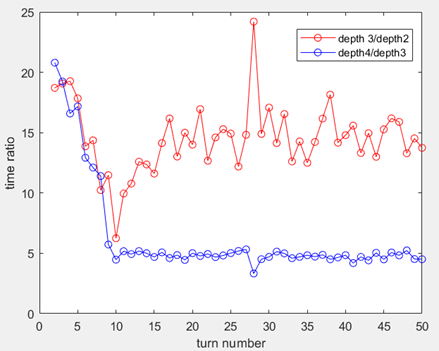
\includegraphics[width=0.6\linewidth]{partE_1}
    \caption{The time ration of two adjacent depths is bound by 25.}
    \label{fig:partE_1}
\end{figure}
